\subsection{Rezonanca sustava bez prigušenja}
Za sustav bez prigušenja, rezonantne frekvencije za $R_d$, $R_v$ i $R_a$ jednake su
prirodnoj frekvenciji sustava što se dobije uvrštavanjem $\zeta = 0$ u \eqref{eq:rd_rezonanca} i 
\eqref{eq:ra_rezonanca}. 
\par

Primjetimo da je maksimalni dinamički koeficijent $R_d$ (za $\omega/\omega_n = 1$) 
neograničen, tj $R_d\to \infty$ što se vidi i u jednadžbi \eqref{eq:fazniSpektarNepriguseno} 
te na grafu \ref{fig:frf-nepriguseno}. U slijedećoj jednadžbi prikazana je vremenska 
funkcija pomaka sustava za homogene početne uvjete:
\begin{equation}
    u(t)=\frac{p_0}{k}\frac{1}{1-(\omega/\omega_n)}
            \left(\sin(\omega t) - \frac{\omega}{\omega_n}\sin(\omega_n t)\right)
\end{equation}

Uočimo da za $\omega = \omega_n$ navedena jednadžba više ne vrijedi (djeljenje s
nulom). Novu jednadžbu možemo odrediti na slijedeći način:
\begin{equation}\label{eq:limes}
    \lim_{\omega\to\omega_n}{u(t)} = 
        \frac{p}{k}\frac{1}{1-(\omega/\omega_n)^2}
            \left(\sin(\omega t) - \frac{\omega}{\omega_n}\sin(\omega_n t)\right)
\end{equation}

Navedeni limes je oblika $\frac{0}{0}$, pa ga je moguće rješiti L'Hopitalovim
pravilom. Deriviranjem funkcije po $\omega$ dobijemo:
\begin{equation}\label{eq:lhopitalovo_limes}
    \lim_{\omega\to\omega_n}\frac{d}{d\omega}u(t)=
    \lim_{\omega\to\omega_n} \left[
        \frac{p_0}{k}\frac{1}{-2(\omega/\omega_n)}
            \left(t\cos(\omega t) - \frac{1}{\omega}\sin(\omega_n t)\right)
           \right]
\end{equation}
Uvrštavanjem $\omega=\omega_n$ dobijemo:
\begin{equation}\label{eq:odziv_rezonanca}
    u(t)=-\frac{1}{2}\frac{p_0}{k}(\omega_n\cos(\omega_n t)-\sin(\omega_nt))
\end{equation}

Iz navedene jednadžbe vidljivo je da usprkos neograničenom dinamičkom faktoru
neizmjerno velika amplituda ne nastupa trenutno, već dolazi do njezinog 
postupnog rasta. Djeljenjem izraza \eqref{eq:odziv_rezonanca} statičkim pomakom i
uvrštavanjem $\omega_n=\frac{2\pi}{T_n}$ dobijemo:
\begin{equation}\label{eq:rezonanca_period}
    \frac{u(t)}{(u_{st})_0}=-\frac{1}{2}
        \left(\frac{2\pi t}{T_n}
                \cos\left(\frac{2\pi t}{T_n}\right)
                -
                \sin\left(\frac{2\pi t}{T_n}\right)
        \right)
\end{equation}
Gdje je:
\begin{table}[H]
    \begin{tabular} {r l}
        $T_n$ & period titranja\\
    \end{tabular}
\end{table}

Iz prethodne jednadžbe slijedi da ekstremi nastupaju svaki poluperiod ($T_n/2$), pri
čemu prvo nastupa maksimum a zatim minimum. Vrijeme nastupa ekstrema za određeni
redni broj titraja prikazuju slijedeće jednadžbe:
\begin{itemize}
    \item za maksimum: $t=(i-\frac{1}{2})T_n$
    \item za minimum: $t=jT_n$
\end{itemize}
Gdje je:
\begin{table}[H]
    \begin{tabular} {r l}
        $t$ & vrijeme nastupa ekstrema\\
        $i$ & redni broj titraja\\
    \end{tabular}
\end{table}
Iznos ekstrema određujemo uvrštavanjem vremena nastupa ekstrema u jednadžbu
\eqref{eq:rezonanca_period} te slijedi:
\begin{enumerate}
    \item iznos maksimuma za j-ti titraj: $u_j=(u_{st})_0\pi(j-\frac{1}{2})$
    \item iznos minimuma za j-ti titraj: $u_j=-(u_{st})_0\pi\cdot j$ 
\end{enumerate}

Prirast maksimuma određujemo razlikom između iznosa maksimuma trenutnog i slijedećeg
titraja što prikazuje slijedeća jednadžba:
\begin{equation}\label{eq:prirast_maksimuma}
    \begin{split}
        |u_{j+1}|-|u_j| &=(u_{st})_0\pi((j+1)-\frac{1}{2})-(u_{st})_0\pi(j-\frac{1}{2})\\
        |u_{j+1}|-|u_j| &= \frac{p_0}{k}\pi
    \end{split}
\end{equation}

Analogno tome određuje se i prirast minimuma koji glasi:
\begin{equation}\label{eq:prirast_minimuma}
    \begin{split}
        u_{j+1}-u_j &= -(u_{st})_0\pi(j+1)-(-(u_{st})_0\pi j)\\
        u_{j+1}-u_j &= -\frac{p_0}{k}\pi
    \end{split}
\end{equation}

Uočimo da su prirasti ekstrema linearni, stoga krivulju ovojnice čine pravaci čiji
su koeficjenti smjera prikazani u nastavku:
\begin{equation}\label{eq:koef_smjera_envelopa}
    k_{1,2}=\pm\frac{1}{2}\frac{p_0}{k}\omega_n
\end{equation}

\begin{figure}[H]
    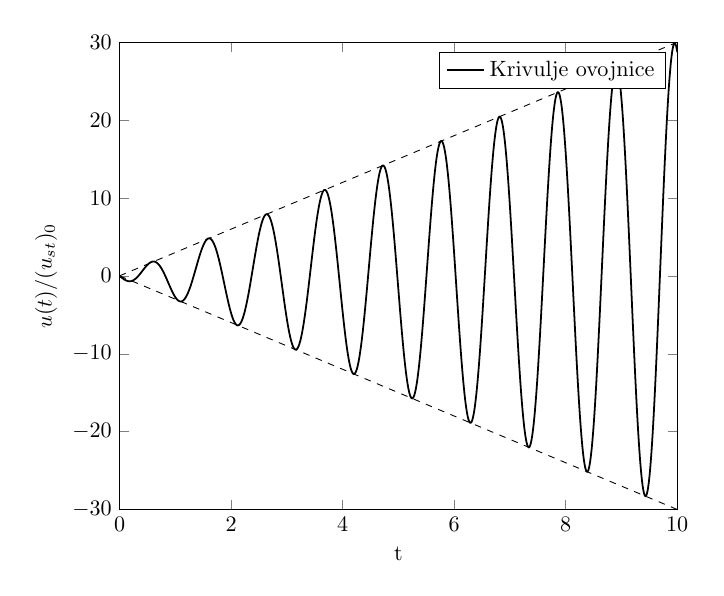
\begin{tikzpicture}[scale=0.8]
    \begin{axis} [
        height=9cm,
%        axis lines = center,
        xlabel=t,ylabel=$u(t)/(u_{st})_0$,
        ylabel near ticks, ylabel style={anchor=south},
        xmin = 0, xmax = 10,
        ymin = -30, ymax =30,
        xtick = {0, 2, 4, 6, 8, 10},
        ytick = {-30,-20,-10,0,10,20,30},
     ]
        \addplot [
            domain=0:10,
            samples=1000,
            color=black,
            thick,
        ] {-0.5*(6*x*cos(6*deg(x))+sin(6*deg(x))};

        \addplot [
            domain=0:10,
            samples=100,
            color=black,
            dashed,
        ] {0.5*6*x};

        \addplot [
            domain=0:10,
            samples=100,
            color=black,
            dashed,
        ] {-0.5*6*x};
        \addlegendentry{Krivulje ovojnice}
    \end{axis}
\end{tikzpicture}

    \label{rezonanca-nepriguseno}
    \caption{Rezonanca neprigusenog sustava}
\end{figure}


